\section{Concrete parameterization}

In order to determine concrete values for the security parameter $m$, we now
turn our attention to a particular adversarial strategy of interest and analyze
its probability of success under specific conditions. It is important to keep
in mind that this adversarial strategy is only one possible strategy and an
advanced adversary can perform more sophisticated attacks. However, the fact
that this attack is reasonable and possible to simulate allows us to extract
specific values for $m$.

The attack is an extension of the stochastic processes originally described in
\cite{bitcoin} and further explored in \cite{rosenfeld}.

The experiment works as follows: Initially, the values $m$ and $k$ are fixed
and some adversarial computational power percentage $q$ over the total network
computational power is chosen. A number of blocks $y$ during which parallel
mining will occur is also fixed. Then the experiment begins with the adversary
and the honest parties sharing a common blockchain which ends in block $B$. As
soon as $B$ is mined, the adversary starts mining in secret and in parallel
with the honest parties on his own private fork on top of $B$. She ignores the
honest chain and does not publish her private fork, so that the two chains
remain disjoint after $B$. As soon as $y$ blocks have been mined in total, the
adversary attempts a double spend by creating two conflicting transactions
which are committed to an honest block and an adversarial block respectively on
top of each current chain. Finally, the adversary mines $k$ blocks on top of
the double spending transaction within her private chain. As soon as these $k$
blocks have been mined, she published her private chain in an attempt to
overcome the honest chain.

Based on the above experiment, we measure the probability of success of the
adversary. Setting $k = 6$ as is common in bitcoin tradition, we experiment
with various values of $m$ for $y = 100$, indicating $100$ blocks of secret
parallel mining. We make the simplifying assumption that honest party
communication is perfect and immediate, meaning that all honest party rounds
that are successful are also uniquely successful. We ran $1,000,000$ Monte
Carlo executions of the experiment for each value of $m$ from $1$ to $30$. We
ran the simulation for values close to the two values of computational power
percentage used in \cite{bitcoin}, $q = 0.1$ and $q = 0.33$. The results are
plotted in Figure~\ref{fig.nipopow-attack-experiment}.

\begin{figure}[h]
    \caption{\label{fig.nipopow-attack-experiment}
        Simulation results for a private mining attacker with $q = 0.1$ and $q
        = 0.33$ computational power, suffix security $k = 6$ and parallel
        mining parameter $y = 100$. Probabilities are plotted on a logarithmic
        scale. The threshold probability of \cite{bitcoin} is indicated in red.
    }
    \centering
    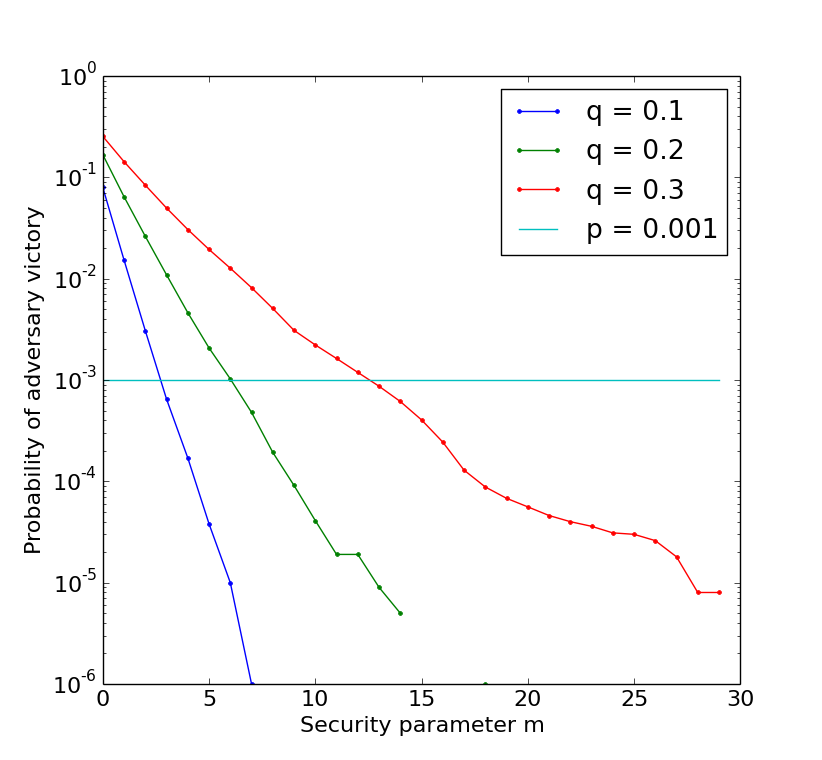
\includegraphics[width=0.5\textwidth,keepaspectratio]{figures/nipopow-attack-experiment.png}
\end{figure}

